
\documentclass[12pt]{report}

\usepackage{CJKutf8}
\usepackage{setspace}
\usepackage{CJK}
%\usepackage{pinyin}

%==
%\usepackage[active]{srcltx}
\usepackage[english]{babel}
\usepackage{amssymb,amsfonts,amsmath}
\usepackage{amsthm}
%\usepackage{fontspec}
\usepackage{mathrsfs}
\usepackage{bm}
\usepackage{url}
\usepackage{graphicx}
\usepackage{xcolor}
\usepackage{t1enc}
\usepackage{comment} 
\usepackage{makeidx}
\usepackage{xspace}
\usepackage{subfigure}
%==
\usepackage[a4paper,left=3cm,top=3cm,right=3cm,bottom=3cm,nohead]{geometry}
\setlength{\baselineskip}{10pt}
\DeclareMathAlphabet{\mathpzc}{OT1}{pzc}{m}{it}

\input{def}

\doublespacing
\pagestyle{plain}
\begin{document}
\onehalfspacing
%\renewcommand{\baselinestretch}{1} 

\begin{titlepage}
\begin{center}

\begin{CJK}{UTF8}{bkai}
\Large{{國立臺灣大學電機資訊學院電機工程學系\\碩士論文}}\\
\large{{Department of Electrical Engineering}}\\
\large{College of Electrical Engineering and Computer Science}\\
\Large{{National Taiwan University}}\\
\Large{{Master Thesis}}\\

\hspace*{1cm}~\\
\hspace*{1cm}~\\
\hspace*{1cm}~\\
\Large{基於Android NFC卡片模擬進行之人性化認證方案\\
A User-friendly Authentication Solution using NFC Card Emulation on Android }\\
\hspace*{1cm}~\\
\hspace*{1cm}~\\
\hspace*{1cm}~\\

\Large{李鎬\\Lee Haw}\\
\hspace*{1cm}~\\
\hspace*{1cm}~\\

\Large{指導教授:鄭振牟 博士\\Advisor: Chen-Mou Cheng, Ph.D.}\\
\hspace*{1cm}~\\
\hspace*{1cm}~\\


\Large{中華民國 103 年 6 月\\June, 2014}\\

\end{CJK}
\end{center}
\end{titlepage}


\clearpage

\pagenumbering{roman}
\setcounter{page}{1}

\doublespacing
\begin{abstract}

With the services provided on the Internet in our daily lives increase dramatically, a secure authentication system becomes more and more important. An insecure authentication system will produce a great threat for users' privacy. In recent years, it is common to see the news of users' credential are stolen by hacking a website's database. In conclusion, the original password-based solution cannot resist to a variety of different attack methods. Usability is important for an authentication system as well. Most of users will not adopt an authentication system no matter how secure it is.

Therefore, this study implements a simple system, based on digital signature algorithm to authenticate the identity of the user to do, and the increasingly widespread use of mobile devices to enhance the convenience and practicality. Finally, we compare this system with the existing system in the viewpoint from security, usability and the deployment ability.


\vspace*{3em}
{\bf Keywords:} \emph{computer security, authentication scheme, digital signature, security and usability, Android host-card-emulation}

\end{abstract}
%\documentclass[12pt]{report}

%\usepackage[a4paper,left=3cm,top=3cm,right=3cm,bottom=2cm,nohead]{geometry}

\doublespacing

%\begin{document}
\onehalfspacing

\begin{titlepage}
\begin{CJK}{UTF8}{bkai}
\begin{center}
\Large{{摘要}}\\
\end{center}

隨著網路上提供的服務在我們日常生活的比例越來越大,認證系統的安全性成為一個很大的問題,一個不安全的認證系統對於使用者的隱私會產生很大的威脅。在近幾年中,某某網站的資料庫被攻擊使得大量的密碼被竊取的新聞屢見不鮮,隨著網路越來越發達,密碼外洩的影響性也越來越大,舊有的帳號密碼機制以無法抵抗各種不同的攻擊手法。認證系統的實用性也是相同重要的,方便使用的系統才容易被使用者接受。

因此,本研究實作了一個簡明的認證系統,藉由數位簽章的機制來對使用者做身分認證,並利用日益廣泛的行動裝置來提昇便利性及實用性,最後將此系統與現有的系統在安全性、便利性以及相容性等方面做了比較。

\vspace*{5em}

{關鍵字:} \emph{電腦安全,認證方案,數位簽章,安全性及實用性,NFC卡片模擬}


\end{CJK}
\end{titlepage}

%\end{document}


\clearpage

\tableofcontents
\listoffigures
\listoftables
\clearpage

\doublespacing
\pagenumbering{arabic}
\setcounter{page}{1}
\setcounter{tocdepth}{1}

%\documentclass[12pt]{article}
%\usepackage{CJK}
%\usepackage{pinyin}

\begin{CJK}{Bg5}{bsmi}

%---------------------------------------------
%	Chapter Introduction
%---------------------------------------------


\chapter{Introduction}

In the age of information, more and more services are provided through the Internet. For these web services, it is important that how to verify users' identity on the web. Therefore, a secure \emph{Authentication System} is essential for each service. Nowadays, the password-based scheme is the most common authenication system. However, it is not secure enough, Malicious attackers can get people's password in many different approaches. [TODO example of attack] Since password-based scheme cannot protect us very well, our privacy are exposed to great danger.

\section{Motivation}

Lots of researchers have demonstrate various authenication methods in recent decades, but some of them are not secure enough. Malicious attackers can get people's password in many different approaches.Moreover, attackers can even steal the private information of users. For example, [TODO example]. Besides, [TODO example] In brief, there are several security weaknesses in the current systems. In brief, several systems have severe security issue.

In addition to the security issue, some system has lower usability. It means that it is not user-frienly. For instance, [TODO example]. In conclusion, these system is hard to use.

According to these reasons mensioned above, the aim of the thesis is to develop a authentication system with high security and usability. I use Digital Signature Algorith to prevent the security issue. Then I take advantage of mobile device to build a user-friendly system.

Compared to existed system, our authentication system is much secure and usable. The rest of the thesis is organized as follows. In chapter 3, I will describe my system more detailed. In chapter 4, I build some criteria to estimate the performance of my authentication system in security, deployment ability, and usability. Then compare it to the password-based scheme. In the last chapter, I compare some existing token-based authentication schemes to my new design, and the proposed system is much useful by comparison.

\end{CJK}
%%% Local Variables: 
%%% mode: latex
%%% TeX-master: "paper"
%%% End: 
    
\begin{CJK}{Bg5}{bsmi}

%---------------------------------------------
%	Chapter Preliminaries
%---------------------------------------------

\chapter{Preliminaries}

\section{Digital Signature Algorithm}

Digital signature is a mathematical scheme for demonstrating the authenticity of a digital message or document. A digital signature scheme typically consists of three algorithms:

\begin{enumerate}
\item[*] A key generation algorithm that selects a private key uniformly at random from a set of possible private keys. The algorithm outputs the private key and a corresponding public key.
\item[*] A signing algorithm that, given a message and a private key, produces a signature.
\item[*] A signature verifying algorithm that, given a message, public key and a signature, either accepts or rejects the message's claim to authenticity.
\end{enumerate}

Digital signatures can be used to authenticate the source of messages. When ownership of a digital signature secret key is bound to a specific user, a valid signature shows that this message is sent from the genuine user. I take the advantage of this authentication property to replace password. In the password-based authentication scheme, the ownership of password is bound to a specific user. 

\section{Near Field Communication}

Near Field Communication (NFC)\cite{nfc-wiki} is a set of standards for smartphones and similar devices to establish radio communication with each other by touching them together or bringing them into proximity, usually no more than a few inches.

Some people may be wondering what is the difference between NFC and Bluetooth. In briefly, NFC technology consumes little power when compared to standard Bluetooth technology\cite{nfc-ble-1}\cite{nfc-ble-2}. The close proximity that devices connected using NFC must be to each other actually proves useful in crowded locations to prevent interference caused when other devices are present and trying to communicate. 

\section{Android HCE Feature}

Many Android devices, which offer NFC functionality, also support card emulation feature. In most cases, this feature is achieved by a separate chip, called \emph{secure element} (SE). The Android system only provides an interface. Therefore, no Android application can involve in the transaction between secure element and the reader. After the transaction complete, an application can query the secure element directly to get transaction status and notify users. This is why the original NFC card emulation functionality also called hardware card emulation.

Because this mechanism needs an extra hardware in devices, most of Android application developers cannot take advantages of card emulation feature. To solve this, Android 4.4 provides an additional method of card emulation, which is not involved with secure element, called \emph{host-base card emulation}. This method allows Android application can communicate with NFC reader directly, and no need the help of extra hardware. Due to this feature, lots of customized NFC application appear, especially for payment, such as Visa and MasterCard\cite{nfc-visa}.

\begin{comment}
\section{OpenID}

OpenID (OID)\cite{openid} is an open standard and decentralized protocol by the non-profit OpenID Foundation that allows users to be authenticated by certain co-operating sites (known as Relying Parties or RP) using a third party service. 

This eliminates the need for webmasters to provide their own ad hoc systems and allowing users to consolidate their digital identities. In other words, users can log into multiple unrelated websites without having to register with their information over and over again. Fig~\ref{fig:openid-flow} is the overview of OpenID protocol and the user flow.
\begin{figure}
\centering
\includegraphics[scale=0.6]{picture/openid-flow.png}
\caption{OpenID overview\cite{openid-flow}}
\label{fig:openid-flow}
\end{figure}
\end{comment}


\section{Existing Solutions}
\label{sec:related-work}

Since researchers have studied authentication system for years, there are several solutions now. I selected four kinds of solution, which is related to hardware-tokens, mobile devices and smart cards. These features are similar to the scheme I proposed, and I'll describe them briefly in the following section.

\subsection{Token-based scheme}

\subsubsection{SecurID}

SecurID, now known as RSA SecurID\cite{rsa-securid}, is a mechanism developed by RSA (the Security Division of EMC) for performing two-factor authentication for a user to a network resource. The following paragraghs will describe how it works simply.

Each device stored a defferent secret \emph{seed}, and the back-end server also know this seed. In every 60 seconds, SecurID will generate an 6-digit authentication code according to its seed, and display on the screen. If a user authenticating to a network service, he has to enter both a personal identification number and the 6-digit code \emph{at that moment}. The server, which also has a real-time clock and a database of valid tokens with the associated seed records, authenticates a user by computing what number the token is supposed to be showing at that moment in time and checking this against what the user entered.

However, in March 2011 attackers compromised RSA's back-end database of seeds\cite{rsa-hack}, which allowed them to predict the authentication codes generated by any token at any time. This attack forces RSA Security to replace almost every one of the 40 million SecurID tokens in use.

\subsubsection{YubiKey}

The YubiKey\cite{yubikey} is another authentication hardware token, which shaped like a USB flash drive. It connects to a USB port and identifies itself as a USB keyboard, which allows it to be compatible to most of computers or laptops with system's native driver. The basic function of the YubiKey is to generate \emph{One-Time Passwords}. 

When users want to authenticating to a network service by YubiKey, after insert YubiKey into the USB port, users have to touch the YubiKey's OTP generation button. The YubiKey will help users typing a string of printable characters-the concatenation of a fixed \emph{identity string} (to replace the username) and a one-time password (to replace the password). Then the verify server will check whether the OTP is valid or not, and check the timestamp to resist to the relay-attack.

\subsection{Mobile-device-based scheme}

\subsubsection{Google 2-step}

Two-step verification is a process involving two stages to verify the identity of an entity trying to access services in a computer or in a network. Google was one of the first Internet companies to introduce a two-step verification process\cite{google-2-step}. 

The first authentication step is just like the original scheme, log in with the username and password. The second step required a mobile phone with SMS service. Users must register his phone number to Google. When a user want to start the 2-step authentication, a text message, which including a one-time code, will send to user's mobile phone via SMS. The user have to enter this code on the website in 30 seconds, or this code will be invalid because of timeout.

\subsection{Smart-card-based scheme}

\subsubsection{Song's Smart-card-based Scheme}

In order to address some of the security and management problems that occur in traditional password-based authentication protocols, researches in recent decades have focused on smart card based password authentication. In 2012, Ronggong Song proposed a new design of smart card based authentication protocol\cite{smart-card}. In his research, he analyzed the previous protocol proposed by Xu-Zhu-Feng and demonstrated a simple improvement. Furthermore, he designed a new strong smart card based authentication protocol. The following fig~\ref{fig:song-smard-card-scheme} shows that how his new scheme works.

\begin{figure}
\centering
\includegraphics[scale=0.4]{picture/song-smart-card-scheme.png}
\caption{Song's amart cart based authentication scheme}
\label{fig:song-smard-card-scheme}
\end{figure}
\end{CJK}
\begin{CJK}{Bg5}{bsmi}

%---------------------------------------------
%	Chapter System Architecture
%---------------------------------------------

\chapter{System Architecture}

In this chapter, I am going to explain my design more detailed. My scheme is based on DSA to provide the security and I'll explain it in the first section. The second section exhibits the user flow in three phases: \emph{register}, \emph{login} and \emph{verification}. The last section presents two demostrations about how to apply this scheme. One is for building a website which support this authentication scheme, the other is for how does this scheme cooperating with the existed website.

\section{System Overview}

Let us recall the autehentication process about the password-based scheme. As the fig~\ref{fig:password-based-flow} shows, the client give his username and password to server, note that the password must to be encrypted because of the security issue. Then the verificaiton server checks whether it is valid according to its database and return the result to user. Figure~\ref{fig:my-scheme-flow} is the authentication process of my scheme. Client should send a login request first, because the verificaiton server is a passive element. After receive a login request, the server will send a nonce, which is composed by the server information and some random bits, back to the client. The client generate a signature for this nonce and return to server. The server use the public key to check whether the client is valid or not.

In comparison to the password-based scheme, my scheme needs two extra steps. But it is not an big issue due to the high data transfer speed of NFC technique. According to this concept, the advantage is that the data communicated between the client and the server do not need to be encrypted. The only \emph{secret} is private key, which is stored in client's storage. The disavantage of my scheme is that users will need to hold a device for creating signature and help them managing their public keys. The next section will offer introduction for each components.
\begin{figure}
\centering
\subfigure[password-based scheme]{
\label{fig:password-based-flow}
\includegraphics[scale=0.6]{picture/password-based-flow.png}
}
\subfigure[my scheme]{
\label{fig:my-scheme-flow}
\includegraphics[scale=0.6]{picture/basic-idea-flow.png}
}
\caption{Authentication flow}
\end{figure}

\begin{figure}
\centering
\includegraphics[scale=0.65]{picture/final-flow.png}
\caption{Authentication flow with mobile device}
\label{fig:final-flow}
\end{figure}

\section{Components and Data flow}

There are 5 parts of my scheme: \emph{Mobile device}, \emph{NFC reader application}, \emph{browser}, \emph{srever} and \emph{its database}, as the figure shows. In this section, I'll introduce the envienment I setup for this system.

\subsubsection{Mobile Device and NFC Channel}

For the mobile device, I use Nesus7 with Android OS (version = 4.4) in my experiments. Android os provide a HostApduService for developers to manage the NFC communication. Specifically, Android 4.4 supports emulating cards that are based on the NFC-Forum ISO-DEP specification (based on ISO/IEC 14443-4) and process Application Protocol Data Units (APDUs) as defined in the ISO/IEC 7816-4 specification. The protocol stack shows as fig~\ref{fig:protocol-stack}. When the user taps a device to an NFC reader, the Android system needs to know which HCE service the NFC reader actually wants to talk to. This is where the ISO/IEC 7816-4 specification comes in: it defines a way to select applications, centered around a 16-bytes Application ID (AID).

\begin{figure}
\centering
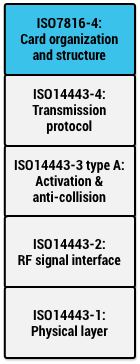
\includegraphics[scale=0.7]{picture/protocol-stack.png}
\caption{Android's HCE protocol stack\cite{nfc-hce-stack}}
\label{fig:protocol-stack}
\end{figure}

\subsubsection{Browser and NFC Reader}
In my setup, it doesn't need a specify browser, some common browser such as Google Chrome, FireFox or even IE can support this scheme. The NFC reader I used is ACR122U. The browser connect to NFC reader through Libnfc\cite{libnfc}, a open-source project about developing NFC-related application.

\subsubsection{Server and its Database}

I use flask, a python framework for web application, for building an verification server in order to proof my concept. I choose to use SQL database, which means my scheme are compatable to password-based scheme. I use HTTP as the transmission protocol. The reason why I don't use HTTP is because of my threat model assumption. I assume that the client side (browser and nfc reader) is unsecure, so even though I adopt HTTPS, the certificate is still untrusted. Thus, I select an unsecure transmission protocol to emphasize that the client-side is untrusted.

\section{User Flow}

In this section, I'll seperate the autentication process into three stages: \emph{register phase}, \emph{login phase} and \emph{verification phase}.

\subsubsection{Register Phase}

\begin{enumerate}
\item Start the initialzization process on his mobile device, that is, set PIN code and generate key pair.
\item User send a registration request to the verification server.
\item Server return the server information to user and pass it to mobile device via reader applicaiton.
\item Mobile device saved the server information and the private key together, and return the device UUID and corresponding public key back to user.
\item User send the id and public key (and other required credentials required by server) to server.
\item Server saved UUID and public key into its database.
\end{enumerate}

In step one, users need to set a PIN code in order to resist to theft. The key pair is generated by RSA in my implementation, but it can be replaced by any asymmetric key encryption algorithm. In step three, the reason why the server has to add server info into the nonce is to resist to the Man-In-The-Middle attack. In step four, I take the device UUID as the identifier instead of the public key is because there are various kinds of DSA, I have to united the ID format for all the users and all the devices.

\subsubsection{Login Phase}

\begin{enumerate}
\item User send a login request to server.
\item Server return a nonce ([server info || random bits]) back to client.
\item The NFC reader start to scan cards as soon as it receive the nonce.
\item User execute the card emulation application on mobile device and enter the PIN code. If the PIN code correct, mobile device enable the HCE mode.
\item Reader application send nonce to mobile device.
\item Mobile device retrieve the server info from nonce, show it on the screen and ask for user's confirmation.
\item Mobile device signed the nonce with corresponding private key.
\item Mobile device pass its UUID and signed-nonce to reader.
\item Client pass these parameters to server.
\end{enumerate}

Note that users have to swipe their device to the NFC reader in 30 seconds right after the reader start scanning. Otherwise, it will send a timeout message to browser. In step nine, verification server is able to ask user to provide some other credentials, but we will not discuss about that because it is not defined in my scheme.

\subsubsection{Verification Phase}

\begin{enumerate}
\item Server retrieve the corresponding public key according to the UUID.
\item Verify the signature with the public key.
\item Return the verification result back to client.
\end{enumerate}

\begin{comment}
\section{Scenario}

\subsection{Future Website}
\label{sec:future-website}

\subsection{Existing Website}

For existing website, it is difficult for them to integrate this scheme with their origin users. Therefore, they can adopt the OpenID protocol to help. Build a verificaiton server with this new scheme and use it to be the \emph{Relying Party} in OpenID protocol.

Take Bitcucket.org as an example, I modified the verificaiton server in section~\ref{sec:future-website} to be an \emph{openid-provider}, that is, to support OpenID feature. When a user need to login to Bitbucket, he have to switch to openid-login mode, enter the server url. Then the authentication process is as same as I described above. 
\end{comment}

\end{CJK}
% \begin{CJK}{Bg5}{bsmi}

%---------------------------------------------
%	Chapter Implementation
%---------------------------------------------
\chapter{Implementation}

\section{Server-Side}

\section{Client-Side}

\section{Android-Side}

\end{CJK}
\begin{CJK}{Bg5}{bsmi}

%---------------------------------------------
%	Chapter Discussion
%---------------------------------------------

\chapter{Discussion}

In this chapter, I'll evaluate my new design's performance in security, deployment ability and usability. Before the security analysis, I determined the threat model, including the secure object, trust boundary and some possible threats. I'll show that my new scheme is more secure than password-based schene under a specify assumption.

In the section of usability analysis and deployment ability analysis, I'll introduce some criterias in order to measure a system's performance. Then I'll show and tell that my design is a user-friendly auuthentication solution for both users and developers.

\section{Security Analysis}

\subsection{Threat Model}

\subsubsection{Secure Object}

\begin{enumerate}
\item[*] Protect user's private credentials.
\end{enumerate}

In my system, the most important goal is to protect user's privacy, that is, attackers cannot pretend to be the real user. To achieve the goal, we cannot leak any information about users' private key. Futhermore, attackers shouldn't get nonce and signed-nonce at same time.

\subsubsection{Trust Boundary}

There are 5 components in this scheme, and 4 possible channels for data transfer, as the fig~\ref{fig:compose-element} shows. Because the mobile device is a private accessories, I assumed that the mobile device is trusted, that is, it is a unrooted Android phone with a secure data storage. No one can dump the memory out or cahnged any value saved in storage. 

\begin{figure}
\centering
\includegraphics[scale=0.6]{picture/compose-element.png}
\caption{Components}
\label{fig:compose-element}
\end{figure}

The browser and the reader applicaiton are usually on the same PC, so we can view these two parts as a same component. Our PC is vulnerable due to spreading virus and malicious program, and sometimes we have to login to some website on a public computer. Our keyboard may be logger. In conclusion, the communication channels between client and either mobile device or server is not secure. Even though I adopt HTTPS for the network channel, the data which transfered on these channel may be sniffed or even modified. The last component is the server side. In my assumption, the server is secure enough, attackers can only read the data saved in the databased but cannot modified them.

Finally, in order to anaysis the threats, we have to assume that the registeration process is secure.

To sum up, my assumption in trust bundary can be arranged as following:
\begin{enumerate}
\item[*] Trusted mobile device with secure storage.
\item[*] The data received during the register phase are all correct.
\item[*] Insecure NFC channel: data might be sniffed.
\item[*] Untrusted browser and NFC reader: data might be sniffed or modified.
\item[*] Insecure internet channel: data changed in plaintext.
\item[*] Secure server and its database: data saved in the database can only be stolen, but can not be modfied.
\end{enumerate}

\subsubsection{Threats}

In this paragraph, I'll discuss the possible threats and weaknesses that could affect my system under this assumption. Futhermore, I'll compare my scheme to the original password-based scheme, to show the improvement of my new design.

First, due to the mobile device is secure, so it is impossible of any attacks on mobile device. Then we considered the attacks on the client side (browser and reader applicaiton). For password-based scheme, malicious people can easily get password by any physically attack such as key-logging attack. 

The network communication is insecure, so this password-based scheme will under phishing attack and the Man-In-The-Middle attack. Next, consider an authetication system with my scheme, all attacks to client side is useless, its because these attack can only get signed-nonce or public key, which do not leak any information about the private key. 

To avoid phishing attack and MITM attack, the nonce generated by server is not composed purely by random bits. The nonce is composed by a 128-bits random number following a nother 128-bits server information. Mobile device can retrieve the server information directly by nonce and show it on the screen. Users have to confirm it before the device generate signature. Moreover, there is another advantage of my scheme. Even though there is an attacker get the authority in one authentication process, the attacker will not be able to use this information on another authentication process. Unlike password-based scheme, if a attacker get your password, then he can pretend to be the real user any time.

Last, for the attacks on the server side. Under my assumption, attackers can only read the data saved in database. For password-based scheme, it is a little dangerous for users. If the users' credentials are saved in plaintext, then the attackers will know everythings he wants. Even though it saved after encrypt, it is still in the risk that the key is found by attackers. To sum up, password-based scheme is still not secure enough under this assumption. Futhermore, user's secret is independent from server to server. Any information leaks from a verification server will not decrease the security of other server. Comparatively, for my scheme, the data saved in server are the UUID and the public key, which cause no any effect to users' privacy.

\section{Usability Analysis}

The usability can not be neglected when researchers trying to design a system.
Usability is a subjective perception, it may be different from person to person.
The following paragragh states the criterias I used to estimate the usability of a system. Then I'll take my new design for example and compare to the password-based scheme.

\subsection{Criterias}

\subsubsection{Memorywise-effort}

This criteria means that how many things a user has to remember when he adopt this scheme. Take password-based scheme as an example, the memorywise-effort is username and password. A scheme with less memorywise effort can get higher score in this criteria.

\subsubsection{Scalable-for-user}

Will this scheme create burden for users? The \emph{scalable} is from the viewpoint of users.

\subsubsection{Nothing-to-carry}

Users do not need to bring anything if they adopt this scheme.

\subsubsection{Physical-effortless}

This criteria means that how many effort should a user do in an authentication process.

\subsubsection{Efficiency}

Efficiency means the during time of an authenticaiton process. Not only the calculating time, it should also include the operating time. For example, if a user need to enter an OTP himself, then this scheme is not efficiency.

\subsubsection{Infrequent-error}

Infrequent-error means this scheme or system must be reliable. It cannot reject an authentication request to a honest user.

\subsubsection{Easy-recovery-from-loss}

Users can regain the authentication ability if they lost their devices or if they forgot the needed credentials.

\subsection{Analysis}

User needs to set a PIN code and remember it in my design, so this scheme is better than password-based scheme from the view point of memory-effort. Second, consider the scalable ability for user, assume that a user want to register 100 account with password-based scheme, he'll need to rebember all the 100 pairs of username and password. In my scheme, the mobile can help user to do that. Thus, the scalable ability of my scheme is better.

The physical effort of password-based scheme is enter username and password. Contrast to my scheme, user only have to swipe their mobile device to the NFC reader. However, some browser can help users to remember their username and password. Thus, in my opinion, these two schemes should get same credit on this criteria. The next two criterias, because there is no any evident problems for efficiency or correctness. There two schemes should get same credit, too.

The last one is easy-recovery-from-loss, there are lots of approach can recovery the password if user forget it. Such as register a backup email address, OTP via SMS and so on. In my scheme, it is obvious that people can not easily recovery his account if he lose his mobile device. To be honestly, all token-based schemes have poor performance in this criteria.

\section{Deployment Ability Analysis}

The deployment ability is also an important thing which is need to be considered, especially in designing an authentication system. A system with high usability means it is friendly to users; a system with high deployment ability means it is friendly to the system provider or, more precise, the developers. The following paragraph states the properties I used to estimate a system's deployment ability.

\subsection{Criterias}

\subsubsection{Accessible}

User who adopt this scheme will not be constrained by disabilities or any other physical conditions.

\subsubsection{User-cost}

The total cost per user of the scheme. It should including both required devices of client-side and required equipment of the verification server.

\subsubsection{Server-compatable}

From the viewpoint of verification server, the scheme is compatable with the text-based passwords. The server will not need change their setup to support this scheme. 

\subsubsection{Browser-compatable}

Users don't have to change anything to support this scheme. 

\subsection{Analysis}

For accessible ability, users will be asked to enter PIN code on mobile device, swipe it to NFC reader and users need to confirm the correctness of server info to ensure the security. Therefore, in my opinion, my scheme doesn't have a good performance of accessible ability.

The total cost of my scheme is the mobile device. The verification server does not need any other equipment. However, because of the high popularity of mobile device, I think it has a not bad performance of user-cost.

It is obvious that my scheme is server-compatable. We can save UUID and public key with text-based format easily. For browser-compatable, users will need a extra reader application rather than password-based scheme, but thwy won't need to change too many things to support this scheme. Thus I think my scheme is server-compatable and a little browser-compatable. 

\end{CJK}
\begin{CJK}{Bg5}{bsmi}

%---------------------------------------------
%	Chapter Conclusion
%---------------------------------------------

\chapter{Conclusion}

\section{Compare to Other Schemes}

\begin{table}[h]
\begin{tabular}{|c|c|c|c|c|c|c|}
\hline
                   & pwd & my scheme & SecurID & YubiKey & Google 2-step & Smard-card \\ \hline
memorywise-effort  & =   &           &         &         &               &            \\ \hline
scalable ability   & =   &           &         &         &               &            \\ \hline
nothing to carry   & =   &           &         &         &               &            \\ \hline
Physical-effort    & =   &           &         &         &               &            \\ \hline
Efficiency         & =   &           &         &         &               &            \\ \hline
Correctness        & =   &           &         &         &               &            \\ \hline
recovery-from-loss & =   &           &         &         &               &            \\ \hline
\end{tabular}
\end{table}

\begin{table}[h]
\begin{tabular}{|c|c|c|c|c|c|c|}
\hline
                   & pwd & my scheme & SecurID & YubiKey & Google 2-step & Smard-card \\ \hline
memorywise-effort  & =   &           &         &         &               &            \\ \hline
scalable ability   & =   &           &         &         &               &            \\ \hline
nothing to carry   & =   &           &         &         &               &            \\ \hline
Physical-effort    & =   &           &         &         &               &            \\ \hline
Efficiency         & =   &           &         &         &               &            \\ \hline
Correctness        & =   &           &         &         &               &            \\ \hline
recovery-from-loss & =   &           &         &         &               &            \\ \hline
\end{tabular}
\end{table}

\begin{table}[h]
\begin{tabular}{|c|c|c|c|c|c|c|}
\hline
                   & pwd & my scheme & SecurID & YubiKey & Google 2-step & Smard-card \\ \hline
memorywise-effort  & =   &           &         &         &               &            \\ \hline
scalable ability   & =   &           &         &         &               &            \\ \hline
nothing to carry   & =   &           &         &         &               &            \\ \hline
Physical-effort    & =   &           &         &         &               &            \\ \hline
Efficiency         & =   &           &         &         &               &            \\ \hline
Correctness        & =   &           &         &         &               &            \\ \hline
recovery-from-loss & =   &           &         &         &               &            \\ \hline
\end{tabular}
\end{table}

\end{CJK}

\printindex

\bibliographystyle{alpha}
\bibliography{nfc_auth_solution}


\end{document}